%********************************************%
%*       Generated from PreTeXt source      *%
%*       on 2026-01-18T21:21:24+01:00       *%
%*   A recent stable commit (2022-07-01):   *%
%* 6c761d3dba23af92cba35001c852aac04ae99a5f *%
%*                                          *%
%*         https://pretextbook.org          *%
%*                                          *%
%********************************************%
\documentclass[oneside,10pt,]{article}
%% Custom Preamble Entries, early (use latex.preamble.early)
%% Default LaTeX packages
%%   1.  always employed (or nearly so) for some purpose, or
%%   2.  a stylewriter may assume their presence
\usepackage{geometry}
\usepackage[version=4]{mhchem}
%% Some aspects of the preamble are conditional,
%% the LaTeX engine is one such determinant
\usepackage{ifthen}
%% etoolbox has a variety of modern conveniences
\usepackage{etoolbox}
\usepackage{ifxetex,ifluatex}
%% Raster graphics inclusion
\usepackage{graphicx}
%% Color support, xcolor package
%% Always loaded, for: add/delete text, author tools
%% Here, since tcolorbox loads tikz, and tikz loads xcolor
\PassOptionsToPackage{dvipsnames,svgnames,table}{xcolor}
\usepackage{xcolor}
%% begin: defined colors, via xcolor package, for styling
%% end: defined colors, via xcolor package, for styling
%% Colored boxes, and much more, though mostly styling
%% skins library provides "enhanced" skin, employing tikzpicture
%% boxes may be configured as "breakable" or "unbreakable"
%% "raster" controls grids of boxes, aka side-by-side
\usepackage{tcolorbox}
\tcbuselibrary{skins}
\tcbuselibrary{breakable}
\tcbuselibrary{raster}
%% We load some "stock" tcolorbox styles that we use a lot
%% Placement here is provisional, there will be some color work also
%% First, black on white, no border, transparent, but no assumption about titles
\tcbset{ bwminimalstyle/.style={size=minimal, boxrule=-0.3pt, frame empty,
colback=white, colbacktitle=white, coltitle=black, opacityfill=0.0} }
%% Second, bold title, run-in to text/paragraph/heading
%% Space afterwards will be controlled by environment,
%% independent of constructions of the tcb title
%% Places \blocktitlefont onto many block titles
\tcbset{ runintitlestyle/.style={fonttitle=\blocktitlefont\upshape\bfseries, attach title to upper} }
%% Spacing prior to each exercise, anywhere
\tcbset{ exercisespacingstyle/.style={before skip={1.5ex plus 0.5ex}} }
%% Spacing prior to each block
\tcbset{ blockspacingstyle/.style={before skip={2.0ex plus 0.5ex}} }
%% xparse allows the construction of more robust commands,
%% this is a necessity for isolating styling and behavior
%% The tcolorbox library of the same name loads the base library
\tcbuselibrary{xparse}
%% The tcolorbox library loads TikZ, its calc package is generally useful,
%% and is necessary for some smaller documents that use partial tcolor boxes
%% See:  https://github.com/PreTeXtBook/pretext/issues/1624
\usetikzlibrary{calc}
%% We use some more exotic tcolorbox keys to restore indentation to parboxes
\tcbuselibrary{hooks}
%% Save default paragraph indentation and parskip for use later, when adjusting parboxes
\newlength{\normalparindent}
\newlength{\normalparskip}
\AtBeginDocument{\setlength{\normalparindent}{\parindent}}
\AtBeginDocument{\setlength{\normalparskip}{\parskip}}
\newcommand{\setparstyle}{\setlength{\parindent}{\normalparindent}\setlength{\parskip}{\normalparskip}}%% Hyperref should be here, but likes to be loaded late
%%
%% Inline math delimiters, \(, \), need to be robust
%% 2016-01-31:  latexrelease.sty  supersedes  fixltx2e.sty
%% If  latexrelease.sty  exists, bugfix is in kernel
%% If not, bugfix is in  fixltx2e.sty
%% See:  https://tug.org/TUGboat/tb36-3/tb114ltnews22.pdf
%% and read "Fewer fragile commands" in distribution's  latexchanges.pdf
\IfFileExists{latexrelease.sty}{}{\usepackage{fixltx2e}}
%% Text height identically 9 inches, text width varies on point size
%% See Bringhurst 2.1.1 on measure for recommendations
%% 75 characters per line (count spaces, punctuation) is target
%% which is the upper limit of Bringhurst's recommendations
\geometry{letterpaper,total={340pt,9.0in}}
%% Custom Page Layout Adjustments (use publisher page-geometry entry)
\geometry{a4paper,total={16cm,25cm}}
%% This LaTeX file may be compiled with pdflatex, xelatex, or lualatex executables
%% LuaTeX is not explicitly supported, but we do accept additions from knowledgeable users
%% The conditional below provides  pdflatex  specific configuration last
%% begin: engine-specific capabilities
\ifthenelse{\boolean{xetex} \or \boolean{luatex}}{%
%% begin: xelatex and lualatex-specific default configuration
\ifxetex\usepackage{xltxtra}\fi
%% realscripts is the only part of xltxtra relevant to lualatex 
\ifluatex\usepackage{realscripts}\fi
%% end:   xelatex and lualatex-specific default configuration
}{
%% begin: pdflatex-specific default configuration
%% We assume a PreTeXt XML source file may have Unicode characters
%% and so we ask LaTeX to parse a UTF-8 encoded file
%% This may work well for accented characters in Western language,
%% but not with Greek, Asian languages, etc.
%% When this is not good enough, switch to the  xelatex  engine
%% where Unicode is better supported (encouraged, even)
\usepackage[utf8]{inputenc}
%% end: pdflatex-specific default configuration
}
%% end:   engine-specific capabilities
%%
%% Fonts.  Conditional on LaTex engine employed.
%% Default Text Font: The Latin Modern fonts are
%% "enhanced versions of the [original TeX] Computer Modern fonts."
%% We use them as the default text font for PreTeXt output.
%% Automatic Font Control
%% Portions of a document, are, or may, be affected by defined commands
%% These are perhaps more flexible when using  xelatex  rather than  pdflatex
%% The following definitions are meant to be re-defined in a style, using \renewcommand
%% They are scoped when employed (in a TeX group), and so should not be defined with an argument
\newcommand{\divisionfont}{\relax}
\newcommand{\blocktitlefont}{\relax}
\newcommand{\contentsfont}{\relax}
\newcommand{\pagefont}{\relax}
\newcommand{\tabularfont}{\relax}
\newcommand{\xreffont}{\relax}
\newcommand{\titlepagefont}{\relax}
%%
\ifthenelse{\boolean{xetex} \or \boolean{luatex}}{%
%% begin: font setup and configuration for use with xelatex
%% Generally, xelatex is necessary for non-Western fonts
%% fontspec package provides extensive control of system fonts,
%% meaning *.otf (OpenType), and apparently *.ttf (TrueType)
%% that live *outside* your TeX/MF tree, and are controlled by your *system*
%% (it is possible that a TeX distribution will place fonts in a system location)
%%
%% The fontspec package is the best vehicle for using different fonts in  xelatex
%% So we load it always, no matter what a publisher or style might want
%%
\usepackage{fontspec}
%%
%% begin: xelatex main font ("font-xelatex-main" template)
%% Latin Modern Roman is the default font for xelatex and so is loaded with a TU encoding
%% *in the format* so we can't touch it, only perhaps adjust it later
%% in one of two ways (then known by NFSS names such as "lmr")
%% (1) via NFSS with font family names such as "lmr" and "lmss"
%% (2) via fontspec with commands like \setmainfont{Latin Modern Roman}
%% The latter requires the font to be known at the system-level by its font name,
%% but will give access to OTF font features through optional arguments
%% https://tex.stackexchange.com/questions/470008/
%% where-and-how-does-fontspec-sty-specify-the-default-font-latin-modern-roman
%% http://tex.stackexchange.com/questions/115321
%% /how-to-optimize-latin-modern-font-with-xelatex
%%
%% end:   xelatex main font ("font-xelatex-main" template)
%% begin: xelatex mono font ("font-xelatex-mono" template)
%% (conditional on non-trivial uses being present in source)
%% end:   xelatex mono font ("font-xelatex-mono" template)
%% begin: xelatex font adjustments ("font-xelatex-style" template)
%% end:   xelatex font adjustments ("font-xelatex-style" template)
%%
%% Extensive support for other languages
\usepackage{polyglossia}
%% Set main/default language based on pretext/@xml:lang value
%% Enable secondary languages based on discovery of @xml:lang values
%% Enable fonts/scripts based on discovery of @xml:lang values
%% Western languages should be ably covered by Latin Modern Roman
%% end:   font setup and configuration for use with xelatex
}{%
%% begin: font setup and configuration for use with pdflatex
%% begin: pdflatex main font ("font-pdflatex-main" template)
\usepackage{lmodern}
\usepackage[T1]{fontenc}
%% end:   pdflatex main font ("font-pdflatex-main" template)
%% begin: pdflatex mono font ("font-pdflatex-mono" template)
%% (conditional on non-trivial uses being present in source)
%% end:   pdflatex mono font ("font-pdflatex-mono" template)
%% begin: pdflatex font adjustments ("font-pdflatex-style" template)
%% end:   pdflatex font adjustments ("font-pdflatex-style" template)
%% end:   font setup and configuration for use with pdflatex
}
%% Micromanage spacing, etc.  The named "microtype-options"
%% template may be employed to fine-tune package behavior
\usepackage{microtype}
%% Symbols, align environment, commutative diagrams, bracket-matrix
\usepackage{amsmath}
\usepackage{amscd}
\usepackage{amssymb}
%% allow page breaks within display mathematics anywhere
%% level 4 is maximally permissive
%% this is exactly the opposite of AMSmath package philosophy
%% there are per-display, and per-equation options to control this
%% split, aligned, gathered, and alignedat are not affected
\allowdisplaybreaks[4]
%% allow more columns to a matrix
%% can make this even bigger by overriding with  latex.preamble.late  processing option
\setcounter{MaxMatrixCols}{30}
%%
%%
%% Division Titles, and Page Headers/Footers
%% titlesec package, loading "titleps" package cooperatively
%% See code comments about the necessity and purpose of "explicit" option.
%% The "newparttoc" option causes a consistent entry for parts in the ToC 
%% file, but it is only effective if there is a \titleformat for \part.
%% "pagestyles" loads the  titleps  package cooperatively.
\usepackage[explicit, newparttoc, pagestyles]{titlesec}
%% The companion titletoc package for the ToC.
\usepackage{titletoc}
%% begin: customizations of page styles via the modal "titleps-style" template
%% Designed to use commands from the LaTeX "titleps" package
\pagestyle{plain}
%% end: customizations of page styles via the modal "titleps-style" template
%%
%% Create globally-available macros to be provided for style writers
%% These are redefined for each occurence of each division
\newcommand{\divisionnameptx}{\relax}%
\newcommand{\titleptx}{\relax}%
\newcommand{\subtitleptx}{\relax}%
\newcommand{\shortitleptx}{\relax}%
\newcommand{\authorsptx}{\relax}%
\newcommand{\epigraphptx}{\relax}%
%% Create environments for possible occurences of each division
%% Environment for a PTX "section" at the level of a LaTeX "section"
\NewDocumentEnvironment{sectionptx}{mmmmmmm}
{%
\renewcommand{\divisionnameptx}{#1}%
\renewcommand{\titleptx}{#2}%
\renewcommand{\subtitleptx}{#3}%
\renewcommand{\shortitleptx}{#4}%
\renewcommand{\authorsptx}{#5}%
\renewcommand{\epigraphptx}{#6}%
\section[{#4}]{#2}%
\label{#7}%
}{}%
%% Environment for a PTX "subsection" at the level of a LaTeX "subsection"
\NewDocumentEnvironment{subsectionptx}{mmmmmmm}
{%
\renewcommand{\divisionnameptx}{#1}%
\renewcommand{\titleptx}{#2}%
\renewcommand{\subtitleptx}{#3}%
\renewcommand{\shortitleptx}{#4}%
\renewcommand{\authorsptx}{#5}%
\renewcommand{\epigraphptx}{#6}%
\subsection[{#4}]{#2}%
\label{#7}%
}{}%
%%
%% Styles for six traditional LaTeX divisions
\titleformat{\part}[display]
{\divisionfont\Huge\bfseries\centering}{\divisionnameptx\space\thepart}{30pt}{\Huge#1}
[{\Large\centering\authorsptx}]
\titleformat{\chapter}[display]
{\divisionfont\huge\bfseries}{\divisionnameptx\space\thechapter}{20pt}{\Huge#1}
[{\Large\authorsptx}]
\titleformat{name=\chapter,numberless}[display]
{\divisionfont\huge\bfseries}{}{0pt}{#1}
[{\Large\authorsptx}]
\titlespacing*{\chapter}{0pt}{50pt}{40pt}
\titleformat{\section}[hang]
{\divisionfont\Large\bfseries}{\thesection}{1ex}{#1}
[{\large\authorsptx}]
\titleformat{name=\section,numberless}[block]
{\divisionfont\Large\bfseries}{}{0pt}{#1}
[{\large\authorsptx}]
\titlespacing*{\section}{0pt}{3.5ex plus 1ex minus .2ex}{2.3ex plus .2ex}
\titleformat{\subsection}[hang]
{\divisionfont\large\bfseries}{\thesubsection}{1ex}{#1}
[{\normalsize\authorsptx}]
\titleformat{name=\subsection,numberless}[block]
{\divisionfont\large\bfseries}{}{0pt}{#1}
[{\normalsize\authorsptx}]
\titlespacing*{\subsection}{0pt}{3.25ex plus 1ex minus .2ex}{1.5ex plus .2ex}
\titleformat{\subsubsection}[hang]
{\divisionfont\normalsize\bfseries}{\thesubsubsection}{1em}{#1}
[{\small\authorsptx}]
\titleformat{name=\subsubsection,numberless}[block]
{\divisionfont\normalsize\bfseries}{}{0pt}{#1}
[{\normalsize\authorsptx}]
\titlespacing*{\subsubsection}{0pt}{3.25ex plus 1ex minus .2ex}{1.5ex plus .2ex}
\titleformat{\paragraph}[hang]
{\divisionfont\normalsize\bfseries}{\theparagraph}{1em}{#1}
[{\small\authorsptx}]
\titleformat{name=\paragraph,numberless}[block]
{\divisionfont\normalsize\bfseries}{}{0pt}{#1}
[{\normalsize\authorsptx}]
\titlespacing*{\paragraph}{0pt}{3.25ex plus 1ex minus .2ex}{1.5em}
%%
%% Styles for five traditional LaTeX divisions
\titlecontents{part}%
[0pt]{\contentsmargin{0em}\addvspace{1pc}\contentsfont\bfseries}%
{\Large\thecontentslabel\enspace}{\Large}%
{}%
[\addvspace{.5pc}]%
\titlecontents{chapter}%
[0pt]{\contentsmargin{0em}\addvspace{1pc}\contentsfont\bfseries}%
{\large\thecontentslabel\enspace}{\large}%
{\hfill\bfseries\thecontentspage}%
[\addvspace{.5pc}]%
\dottedcontents{section}[3.8em]{\contentsfont}{2.3em}{1pc}%
\dottedcontents{subsection}[6.1em]{\contentsfont}{3.2em}{1pc}%
\dottedcontents{subsubsection}[9.3em]{\contentsfont}{4.3em}{1pc}%
%%
%% Begin: Semantic Macros
%% To preserve meaning in a LaTeX file
%%
%% \mono macro for content of "c", "cd", "tag", etc elements
%% Also used automatically in other constructions
%% Simply an alias for \texttt
%% Always defined, even if there is no need, or if a specific tt font is not loaded
\newcommand{\mono}[1]{\texttt{#1}}
%%
%% Following semantic macros are only defined here if their
%% use is required only in this specific document
%%
%% Used for warnings, typically bold and italic
\newcommand{\alert}[1]{\textbf{\textit{#1}}}
%% End: Semantic Macros
%% Equation Numbering
%% Controlled by  numbering.equations.level  processing parameter
%% No adjustment here implies document-wide numbering
\numberwithin{equation}{section}
%% "tcolorbox" environment for a single image, occupying entire \linewidth
%% arguments are left-margin, width, right-margin, as multiples of
%% \linewidth, and are guaranteed to be positive and sum to 1.0
\tcbset{ imagestyle/.style={bwminimalstyle} }
\NewTColorBox{tcbimage}{mmm}{imagestyle,left skip=#1\linewidth,width=#2\linewidth}
%% Wrapper environment for tcbimage environment with a fourth argument
%% Fourth argument, if nonempty, is a vertical space adjustment
%% and implies image will be preceded by \leavevmode\nopagebreak
%% Intended use is for alignment with a list marker
\NewDocumentEnvironment{image}{mmmm}{\notblank{#4}{\leavevmode\nopagebreak\vspace{#4}}{}\begin{tcbimage}{#1}{#2}{#3}}{\end{tcbimage}%
}%% For improved tables
\usepackage{array}
%% Some extra height on each row is desirable, especially with horizontal rules
%% Increment determined experimentally
\setlength{\extrarowheight}{0.2ex}
%% Define variable thickness horizontal rules, full and partial
%% Thicknesses are 0.03, 0.05, 0.08 in the  booktabs  package
\newcommand{\hrulethin}  {\noalign{\hrule height 0.04em}}
\newcommand{\hrulemedium}{\noalign{\hrule height 0.07em}}
\newcommand{\hrulethick} {\noalign{\hrule height 0.11em}}
%% We preserve a copy of the \setlength package before other
%% packages (extpfeil) get a chance to load packages that redefine it
\let\oldsetlength\setlength
\newlength{\Oldarrayrulewidth}
\newcommand{\crulethin}[1]%
{\noalign{\global\oldsetlength{\Oldarrayrulewidth}{\arrayrulewidth}}%
\noalign{\global\oldsetlength{\arrayrulewidth}{0.04em}}\cline{#1}%
\noalign{\global\oldsetlength{\arrayrulewidth}{\Oldarrayrulewidth}}}%
\newcommand{\crulemedium}[1]%
{\noalign{\global\oldsetlength{\Oldarrayrulewidth}{\arrayrulewidth}}%
\noalign{\global\oldsetlength{\arrayrulewidth}{0.07em}}\cline{#1}%
\noalign{\global\oldsetlength{\arrayrulewidth}{\Oldarrayrulewidth}}}
\newcommand{\crulethick}[1]%
{\noalign{\global\oldsetlength{\Oldarrayrulewidth}{\arrayrulewidth}}%
\noalign{\global\oldsetlength{\arrayrulewidth}{0.11em}}\cline{#1}%
\noalign{\global\oldsetlength{\arrayrulewidth}{\Oldarrayrulewidth}}}
%% Single letter column specifiers defined via array package
\newcolumntype{A}{!{\vrule width 0.04em}}
\newcolumntype{B}{!{\vrule width 0.07em}}
\newcolumntype{C}{!{\vrule width 0.11em}}
%% tcolorbox to place tabular outside of a sidebyside
\tcbset{ tabularboxstyle/.style={bwminimalstyle,} }
\newtcolorbox{tabularbox}[3]{tabularboxstyle, left skip=#1\linewidth, width=#2\linewidth,}
%% More flexible list management, esp. for references
%% But also for specifying labels (i.e. custom order) on nested lists
\usepackage{enumitem}
%% hyperref driver does not need to be specified, it will be detected
%% Footnote marks in tcolorbox have broken linking under
%% hyperref, so it is necessary to turn off all linking
%% It *must* be given as a package option, not with \hypersetup
\usepackage[hyperfootnotes=false]{hyperref}
%% configure hyperref's  \href{}{}  and  \nolinkurl  to match listings' inline verbatim
\renewcommand\UrlFont{\small\ttfamily}
%% Hyperlinking active in electronic PDFs, all links without surrounding boxes and blue
\hypersetup{colorlinks=true,linkcolor=blue,citecolor=blue,filecolor=blue,urlcolor=blue}
%% Less-clever names for hyperlinks are more reliable, *especially* for structural parts
%% See comments in the code to learn more about the importance of this setting
\hypersetup{hypertexnames=false}
%%The  hypertexnames  setting then confuses the hyperlinking from the index
%%This patch resolves the incorrect links, see code for StackExchange post.
\makeatletter
\patchcmd\Hy@EveryPageBoxHook{\Hy@EveryPageAnchor}{\Hy@hypertexnamestrue\Hy@EveryPageAnchor}{}{\fail}
\makeatother
\hypersetup{pdftitle={Résonance Paramagnétique Electronique}}
%% If you manually remove hyperref, leave in this next command
%% This will allow LaTeX compilation, employing this no-op command
\providecommand\phantomsection{}
%% Division Numbering: Chapters, Sections, Subsections, etc
%% Division numbers may be turned off at some level ("depth")
%% A section *always* has depth 1, contrary to us counting from the document root
%% The latex default is 3.  If a larger number is present here, then
%% removing this command may make some cross-references ambiguous
%% The precursor variable $numbering-maxlevel is checked for consistency in the common XSL file
\setcounter{secnumdepth}{3}
%%
%%
%% A faux tcolorbox whose only purpose is to provide common numbering
%% facilities for most blocks (possibly not projects, 2D displays)
%% Controlled by  numbering.theorems.level  processing parameter
\newtcolorbox[auto counter, number within=section]{block}{}
%%
%% This document is set to number PROJECT-LIKE on a separate numbering scheme
%% So, a faux tcolorbox whose only purpose is to provide this numbering
%% Controlled by  numbering.projects.level  processing parameter
\newtcolorbox[auto counter, number within=section]{project-distinct}{}
%% A faux tcolorbox whose only purpose is to provide common numbering
%% facilities for 2D displays which are subnumbered as part of a "sidebyside"
\makeatletter
\newtcolorbox[auto counter, number within=tcb@cnt@block, number freestyle={\noexpand\thetcb@cnt@block(\noexpand\alph{\tcbcounter})}]{subdisplay}{}
\makeatother
%%
%% tcolorbox, with styles, for REMARK-LIKE
%%
%% remark: fairly simple numbered block/structure
\tcbset{ remarkstyle/.style={bwminimalstyle, runintitlestyle, blockspacingstyle, after title={\space}, before upper app={\setparstyle}, } }
\newtcolorbox[use counter from=block]{remark}[3]{title={{#1~\thetcbcounter\notblank{#2}{\space\space#2}{}}}, phantomlabel={#3}, breakable, after={\par}, remarkstyle, }
%%
%% xparse environments for introductions and conclusions of divisions
%%
%% introduction: in a structured division
\NewDocumentEnvironment{introduction}{m}
{\notblank{#1}{\noindent\textbf{#1}\space}{}}{\par\medskip}
%% Graphics Preamble Entries
%% If tikz has been loaded, replace ampersand with \amp macro
%% Custom Preamble Entries, late (use latex.preamble.late)
%% extpfeil package for certain extensible arrows,
%% as also provided by MathJax extension of the same name
%% NB: this package loads mtools, which loads calc, which redefines
%%     \setlength, so it can be removed if it seems to be in the 
%%     way and your math does not use:
%%     
%%     \xtwoheadrightarrow, \xtwoheadleftarrow, \xmapsto, \xlongequal, \xtofrom
%%     
%%     we have had to be extra careful with variable thickness
%%     lines in tables, and so also load this package late
\usepackage{extpfeil}
%% Begin: Author-provided macros
%% (From  docinfo/macros  element)
%% Plus three from PTX for XML characters

\newcommand{\lt}{<}
\newcommand{\gt}{>}
\newcommand{\amp}{&}
%% End: Author-provided macros
%% Title page information for article
\title{Résonance Paramagnétique Electronique}
\author{Jérôme Estève, Pierre Grégoire
}
\date{}
\begin{document}
%% bottom alignment is explicit, since it normally depends on oneside, twoside
\raggedbottom
%% Target for xref to top-level element is document start
\hypertarget{shorttitlelowercase}{}
\maketitle
\thispagestyle{empty}

\section*{Avant-propos}
L'objectif de la séance est de mettre en évidence le phénomène de résonance paramagnétique électronique. Ce phénomène, également appelé résonance de spin électronique ou Electron Paramagnetic Resonance (EPR) en anglais, est une technique de spectroscopie utilisée pour étudier les espèces chimiques possédant des électrons non appariés. Elle est particulièrement adaptée à l’analyse des radicaux libres, des ions de métaux de transition et de certains défauts paramagnétiques dans les solides. Le principe de la RPE repose sur l’interaction entre le moment magnétique de l’électron et un champ magnétique externe. Lorsqu’un échantillon paramagnétique est soumis à ce champ et irradié par des micro-ondes, une transition entre les niveaux d’énergie des spins électroniques se produit lorsque la condition de résonance%
\begin{gather*}
h \nu = g \mu_B B 
\end{gather*}
est satisfaite. Dans cette formule, \(g\) est le rapport gyromagnétique de l'électron (ou facteur de Landé) et \(\mu_B\) est le magnéton de Bohr. Pour un électron dans le vide, \(g \approx 2\) et la fréquence de résonance est d'environ 2.8 MHz\slash{}G.%
\par
Pour observer cette résonance, nous allons coupler les spins électroniques à un résonateur diélectrique réalisé en \(\ce{KTaO3}\) (KTO), un matériau de grande constante diélectrique (\(\epsilon_r \approx 300\)), et observer la modification de la résonance induite par la présence des spins. Lorsqu'on augmente le champ magnétique, la fréquence de résonance des spins augmente et on observe un croisement évité lorsqu'elle traverse celle du résonateur.%
\par
Le TP se déroule en trois parties:%
\begin{itemize}[label=\textbullet]
\item{}Dans la première partie, l'objectif est d'apprendre à manipuler un analyseur de réseau vectoriel (VNA) qui est un instrument de mesure fondamental en ingénierie micro-ondes. Ici, on utilise le VNA pour caractériser le résonateur diélectrique en KTO.%
\item{}Dans la deuxième partie, on réalise un montage dit de Pound-Drever-Hall permettant de suivre en temps réel la fréquence de résonance du résonateur.%
\item{}Enfin dans la troisième partie, le résonateur en KTO est couplé à des spins électroniques afin d'observer la résonance de spin.%
\end{itemize}
%
\par
Ce document vous guidera tout au long du TP. Vous utiliserez un notebook Jupyter pour acquérir des données sur l'ordinateur et les enregistrer. Vous placerez vos fichiers dans le répertoire correspondant à votre groupe qui est accessible \href{http://localhost:8888/lab/tree/}{ici}.%
\par
\vspace{0.5cm}
\alert{Afin de ne pas endommager le matériel mis à votre disposition, nous vous demandons de faire attention aux trois points suivants:}%
\begin{itemize}[label=\textbullet]
\item{}Toujours utiliser la clé dynamométrique pour serrer un câble SMA, et ne pas serrer au-delà du couple réglé sur la clé.%
\item{}Ne pas envoyer plus que 1 mW de puissance micro-onde sur la diode de détection.%
\item{}Ne pas faire tomber le résonateur en KTO qui est petit, transparent et se perd vite...%
\end{itemize}

\newpage
%
%
%
\typeout{************************************************}
\typeout{Section 1 Résonateur diélectrique en KTO}
\typeout{************************************************}
%
\begin{sectionptx}{Section}{Résonateur diélectrique en KTO}{}{Résonateur diélectrique en KTO}{}{}{section-1}
\begin{introduction}{}%
Dans cette première partie, l'objectif est de caractériser le résonateur diélectrique qui sera utilisé dans la troisième partie pour observer la résonance de spin. Pour observer la résonance qui se situe dans le domaine micro-ondes (entre 7 et 8 GHz), on utilise un analyseur de réseau vectoriel, en anglais Vector Network Analyzer (VNA).%
\end{introduction}%
%
%
\typeout{************************************************}
\typeout{Sous-section 1.1 Analyseur de réseau (VNA)}
\typeout{************************************************}
%
\begin{subsectionptx}{Sous-section}{Analyseur de réseau (VNA)}{}{Analyseur de réseau (VNA)}{}{}{subsec-}
Un analyseur de réseau vectoriel permet de mesurer les paramètres de scattering \(S_{ij}\) d'un dispositif micro-ondes à un ou deux ports.%
\begin{image}{0.25}{0.5}{0.25}{}%
\includegraphics[width=\linewidth]{external/scattering.pdf}
\end{image}%
La matrice de scattering \(S_{ij}\) relie les amplitudes diffusées aux amplitudes incidentes%
\begin{align*}
\begin{pmatrix} a_{1}^\text{out} \\ a_{2}^\text{out} \end{pmatrix} = \begin{pmatrix} S_{11} \amp S_{12} \\ S_{21} \amp S_{22} \end{pmatrix}  \begin{pmatrix} a_{1}^\text{in} \\ a_{2}^\text{in} \end{pmatrix} 
\end{align*}
%
\par
L'analyseur peut mesurer à la fois les coefficients de réflexion \(S_{ii}\) et de transmission \(S_{i \neq j}\). En général \(S_{12}=S_{21}\), mais ce n'est pas forcément le cas. Pour mesurer, par exemple \(S_{12}\), l'appareil émet un signal par le port 2 et mesure le signal sur le port 1. Le VNA mesure le module et la phase de chaque paramètre \(S_{ij}\) en fonction de la fréquence.%
\par
Les paramètres les plus importants à régler pour la mesure sont:%
\begin{itemize}[label=\textbullet]
\item{}le "span", c'est à dire l'étendue du domaine de fréquence \(\Delta f\) qui est balayé pendant un sweep%
\item{}le nombre de points \(N\) dans le sweep en fréquence qui fixe l'écart \(\delta f = \Delta f/N\) entre deux points de mesure%
\item{}la largeur de bande (Resolution Bandwidth, "RBW") qui fixe le temps d'intégration (\(1/\text{RBW}\)) pour chaque point de mesure%
\item{}la puissance émise par le VNA pour effectuer la mesure ("Power")%
\end{itemize}
%
\end{subsectionptx}
%
%
\typeout{************************************************}
\typeout{Sous-section 1.2 Calibration du VNA}
\typeout{************************************************}
%
\begin{subsectionptx}{Sous-section}{Calibration du VNA}{}{Calibration du VNA}{}{}{subsection-calibration}
Avant d'utiliser le VNA pour caractériser un élément, il faut effectuer une calibration afin de s'affranchir de la propagation dans les câbles entre le VNA et le dispositif à caractériser. Pour effectuer cette calibration, on applique des standards (open, short, match) sur chaque port, puis on mesure la transmission entre les deux ports (through).%
\begin{itemize}[label=\textbullet]
\item{}Branchez deux câbles SMA sur les deux ports du VNA et connectez les deux câbles avec un I. Appuyez sur "Preset" pour appliquer les paramètres de mesure par défaut.%
\item{}Explorez les menus "Measurement" et "Format" pour mesurer et afficher le module et la phase ou la partie réelle et imaginaire de différents paramètres de scattering.%
\item{}Observez le signal mesuré en transmission \(S_{12}\) et en réflexion (\(S_{11}\) ou \(S_{22}\)). Comparez au signal attendu pour un montage idéal.%
\item{}Enlevez le I, et effectuez la calibration "TOSM" en appuyant sur la touche "CAL". Suivez les instructions et branchez chaque élément du kit de calibration sur chaque câble avant de lancer la mesure.%
\item{}Enlevez le dispositif de calibration et observez à nouveau les coefficients de réflexion en phase et module. Qu'observez-vous ?%
\item{}Connectez à nouveau les deux câbles avec un I et observez la transmission en phase et module. Qu'observez-vous ?%
\item{}Remplacez le I par le guide microstrip sur le porte-échantillon. Comment évolue la phase avec la fréquence ? En déduire la vitesse de propagation dans le guide du porte-échantillon. On pourra acquérir une trace et en faire l'analyse dans un notebook Jupyter.%
\item{}Utilisez la fonction "Auto length" dans le menu "Offset" pour compenser la propagation dans le guide. Le dispositif est maintenant calibré.%
\end{itemize}
%
\end{subsectionptx}
%
%
\typeout{************************************************}
\typeout{Sous-section 1.3 Caractérisation du résonateur en KTO}
\typeout{************************************************}
%
\begin{subsectionptx}{Sous-section}{Caractérisation du résonateur en KTO}{}{Caractérisation du résonateur en KTO}{}{}{subsec-resonator-coupling}
On utilise un résonateur parallélépipédique en KTO de dimensions 5x5x0.5 mm. Le KTO est un matériau paraélectrique proche de la transition ferroélectrique. Il est donc très facilement polarisable et sa constante diélectrique est très élevée, environ 300 à température ambiante et 4000 à basse température. Comme l'épaisseur du résonateur est bien plus petite que ses dimensions transverses, on peut considérer le KTO comme un guide planaire. Les modes propres sont alors les ondes stationnaires d'un résonateur carré. Le mode fondamental est le mode TE01 dont le champ magnétique ressemble à celui d'un dipôle magnétique. La figure ci-dessous montre l'intensité et les lignes de champ magnétique:%
\begin{image}{0.25}{0.5}{0.25}{}%
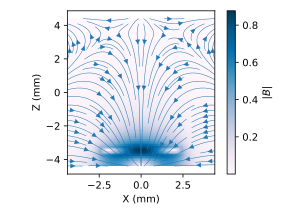
\includegraphics[width=\linewidth]{external/KTO_TE01_mag_field_lines.pdf}
\end{image}%
L'intérêt principal de ce résonateur de grande constante diélectrique est d'obtenir un champ magnétique micro-ondes intense à la surface du résonateur. Pour exciter les modes de résonance, il suffit de placer le KTO près du guide d'onde sur le porte-échantillon.%
\par
%
\begin{itemize}[label=\textbullet]
\item{}Placez le résonateur près du guide et observez la transmission au VNA entre 7 et 8 GHz.%
\item{}Comment varie la résonance avec la distance au guide ?%
\end{itemize}
%
\par
Pour comprendre l'évolution de la résonance, on introduit le taux de perte par couplage \(\kappa_c\) et le taux de perte intrinsèque \(\kappa_i\). Les pertes totales sont \(\kappa=\kappa_c+\kappa_i\), l'énergie stockée dans le résonateur décroît comme \(\exp (-\kappa t)\) avec le temps. On distingue deux régimes limites: le régime sur-couplé \(\kappa_c \gg \kappa_i\) et le régime sous-couplé \(\kappa_c \ll \kappa_i\).%
\begin{itemize}[label=\textbullet]
\item{}Sans faire de calcul, essayez de tracer \(S_{12}\), \(S_{13}\) et \(S_{33}\) dans chaque régime. Les numéros des ports sont définis sur le schéma ci-dessous:%
\end{itemize}
%
\begin{image}{0.25}{0.5}{0.25}{}%
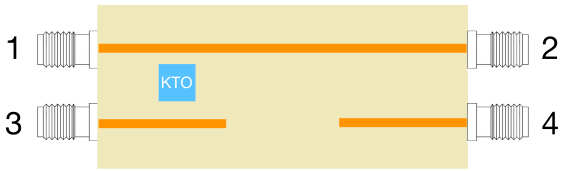
\includegraphics[width=\linewidth]{external/sample_holder.pdf}
\end{image}%
%
\begin{itemize}[label=\textbullet]
\item{}Effectuez les mesures au VNA pour vérifier vos prédictions. Enregistrez quelques traces au format HDF5 qui vous serviront à illustrer votre rapport et essayez d'estimer \(\kappa_i\) pour le résonateur.%
\end{itemize}
%
\par
Pour mesurer la résonance de spin, on cherche à mesurer le plus précisément possible la fréquence de résonance du résonateur.%
\begin{itemize}[label=\textbullet]
\item{}Dans quel régime de couplage faut-il se placer ?%
\item{}Trouvez une configuration où ce régime est à peu près atteint pour la mesure \(S_{12}\).%
\end{itemize}
%
\end{subsectionptx}
\end{sectionptx}
%
%
\typeout{************************************************}
\typeout{Section 2 Montage Pound-Drever-Hall}
\typeout{************************************************}
%
\begin{sectionptx}{Section}{Montage Pound-Drever-Hall}{}{Montage Pound-Drever-Hall}{}{}{section-2}
\begin{introduction}{}%
Le montage de Pound-Drever-Hall est surtout utilisé en optique pour asservir un laser sur une cavité. Il peut être adapté au régime micro-onde avec une source et un résonateur. A la résonance, l'intensité du signal transmis ou réfléchi par le résonateur présente un extremum avec une dérivée nulle. La méthode développée par Pound, Drever et Hall permet d'obtenir un signal d'erreur qui passe par zéro lorsque la fréquence de la source traverse celle du résonateur. Une description détaillée de la technique est disponible sur la page \href{https://en.wikipedia.org/wiki/Pound\%E2\%80\%93Drever\%E2\%80\%93Hall_technique}{Wikipedia dédiée}. La méthode est utilisée le plus souvent en réflexion mais fonctionne également en transmission.%
\begin{image}{0.05}{0.9}{0.05}{}%
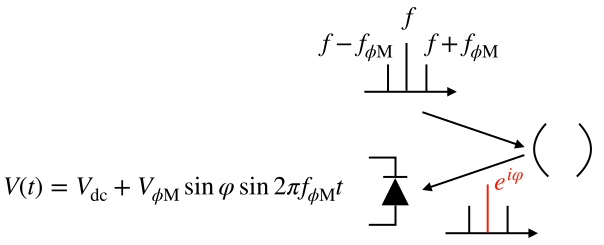
\includegraphics[width=\linewidth]{external/pdh_principle.pdf}
\end{image}%
Pour obtenir un signal d'erreur, la source est modulée en phase à une fréquence \(f_{\phi\text{M}}\). Le signal arrivant sur le résonateur contient trois fréquences: une porteuse à \(f\) et deux bandes latérales à \(f \pm f_{\phi\text{M}}\). En notation complexe, l'amplitude émise par la source s'écrit:%
\begin{gather*}
A^{\text{in}} = A_0 e^{2i\pi f t} (1 + \epsilon \, e^{2i\pi f_{\phi\text{M}} t} - \epsilon  \, e^{2i\pi f_{\phi\text{M}} t}  ) 
\end{gather*}
Notez bien la présence du signe moins entre les amplitudes des deux bandes latérales. On suppose que le taux de perte du résonateur est uniquement dû au couplage par le port de mesure. Le coefficient de réflexion est alors de module unité et les trois composantes subissent juste un déphasage à la réflexion. Si l'on suppose que \(f_{\phi\text{M}} \gg \kappa\), les bandes latérales ne voient pas la résonance et ne sont donc pas déphasées. L'amplitude réfléchie est%
\begin{gather*}
A^{\text{ref}} = A_0  e^{2i\pi f t} (e^{i \varphi} + \epsilon \, e^{2i\pi f_{\phi\text{M}} t} - \epsilon \, e^{2i\pi f_{\phi\text{M}} t}  ) 
\end{gather*}
Au premier ordre en \(\epsilon\), la puissance réfléchie est%
\begin{gather*}
P^{\text{ref}} = \frac{1}{2} (1+4 \epsilon \sin \varphi \sin 2\pi f_{\phi\text{M}} t) 
\end{gather*}
On voit donc que la phase \(\varphi\), qui passe par zéro à la résonance, peut être mesurée en démodulant la tension en sortie de la diode à la fréquence \(f_{\phi\text{M}}\). Le signe moins entre bandes latérales permet d'obtenir \(\sin \varphi\) (et non \(\cos \varphi\)). Pour un montage en transmission, comme considéré ci-dessous, le maximum de variation de la phase est obtenu pour \(\kappa_c=\kappa_i\). On a alors%
\begin{gather*}
\varphi = \frac{2\pi \epsilon (f-f_0)}{\kappa_i} 
\end{gather*}
%
\end{introduction}%
%
%
\typeout{************************************************}
\typeout{Sous-section 2.1 Schéma du montage}
\typeout{************************************************}
%
\begin{subsectionptx}{Sous-section}{Schéma du montage}{}{Schéma du montage}{}{}{sec-montage}
\begin{image}{0.125}{0.75}{0.125}{}%
\includegraphics[width=\linewidth]{external/pdh_setup_1.pdf}
\end{image}%
%
\begin{itemize}[label=\textbullet]
\item{}Réalisez le montage ci-dessus, l'élément à gauche, en sortie du porte-échantillon, est la diode permettant de détecter la puissance du signal micro-onde. La tension en sortie est proportionnelle à la puissance micro-onde en entrée. Il ne faut pas dépasser 0 dBm en entrée et la zone de fonctionnement linéaire se situe en dessous de -10 dBm.%
\item{}Programmez un sweep en fréquence sur la source micro-onde et observez la résonance en mesurant la tension à la sortie de la diode. Vous devez observer un pic de tension, comparable à la mesure obtenue en module avec le VNA.%
\end{itemize}
%
\par
Pour obtenir un signal d'erreur, il faut moduler en phase la source et démoduler le signal en sortie de la diode de détection. Pour cela, on utilise une détection synchrone (lock-in), ici un HF2LI de Zürich Instruments.%
\begin{image}{0.125}{0.75}{0.125}{}%
\includegraphics[width=\linewidth]{external/pdh_setup_2.pdf}
\end{image}%
%
\begin{itemize}[label=\textbullet]
\item{}Modifiez le montage comme ci-dessus pour brancher la modulation du lock-in à \(f_{\phi\text{M}}\) sur l'entrée externe de la source micro-onde et la sortie de la diode sur l'entrée de mesure du lock-in.%
\item{}Programmez la source micro-onde pour obtenir une modulation en phase pilotée par l'entrée externe. Utilisez le mode \(\phi\text{M}\) High Bandwidth et réglez l'amplitude de modulation de phase au maximum.%
\end{itemize}
%
\end{subsectionptx}
%
%
\typeout{************************************************}
\typeout{Sous-section 2.2 Réglage du lock-in}
\typeout{************************************************}
%
\begin{subsectionptx}{Sous-section}{Réglage du lock-in}{}{Réglage du lock-in}{}{}{subsec-lock-in}
L'interface de contrôle du lock-in est accessible \href{https://localhost:8006}{ici}.%
\begin{itemize}[label=\textbullet]
\item{}Programmez le lock-in pour effectuer une mesure à \(f_{\phi\text{M}}\) de l'ordre de quelques MHz (typiquement 2 MHz), utilisez une amplitude de modulation de 1 Vpp maximum.%
\item{}Réglez la démodulation jusqu'à observer un signal d'erreur lorsque la source effectue un sweep en fréquence.%
\item{}Programmez le lock-in pour envoyer le résultat de la démodulation sur la voie auxiliaire 1 afin de pouvoir l'observer sur l'oscillo.%
\item{}Optimisez les paramètres, fréquence, déphasage, amplitude de modulation, position du KTO... pour maximiser l'amplitude du signal d'erreur.%
\item{}Enregistrez quelques traces d'oscillo montrant les différents signaux en fonction de la rampe de fréquence.%
\item{}Estimez la sensibilité de la mesure de la résonance%
\end{itemize}
%
\end{subsectionptx}
\end{sectionptx}
%
%
\typeout{************************************************}
\typeout{Section 3 Observation de la résonance de spin}
\typeout{************************************************}
%
\begin{sectionptx}{Section}{Observation de la résonance de spin}{}{Observation de la résonance de spin}{}{}{section-3}
\begin{introduction}{}%
Pour observer la résonance de spin, on dispose d'un électroaimant pouvant générer un champ magnétique variable entre 0 et 1 T. En plaçant un matériau contenant des spins non appariés à la surface du résonateur au centre de l'aimant et en ajustant le champ magnétique, on s'attend à observer une modification de la résonance détectée avec le montage Pound-Drever-Hall lorsque la fréquence de résonance des spins \(g\mu_B B/h\) coincide avec celle du résonateur.%
\par
Pour améliorer la sensibilité de la mesure, on réalise un deuxième montage de détection synchrone. Le champ magnétique est modulé à environ 100 Hz et on démodule à cette fréquence le signal de sortie du montage Pound-Drever-Hall (PDH).%
\end{introduction}%
%
%
\typeout{************************************************}
\typeout{Sous-section 3.1 Calibration de l'aimant}
\typeout{************************************************}
%
\begin{subsectionptx}{Sous-section}{Calibration de l'aimant}{}{Calibration de l'aimant}{}{}{subsec-magnet}
%
\begin{itemize}[label=\textbullet]
\item{}A l'aide du gauss-mètre, mesurez l'intensité du champ magnétique au centre de l'aimant pour quelques valeurs de courant. Tracez la courbe de calibration de l'aimant.%
\item{}Estimez le champ magnétique permettant de mettre les spins en résonance avec le mode du résonateur et le courant correspondant à mettre dans les bobines.%
\end{itemize}
%
\end{subsectionptx}
%
%
\typeout{************************************************}
\typeout{Sous-section 3.2 Montage à double détection synchrone}
\typeout{************************************************}
%
\begin{subsectionptx}{Sous-section}{Montage à double détection synchrone}{}{Montage à double détection synchrone}{}{}{subsec-ddlockin}
%
\begin{itemize}[label=\textbullet]
\item{}Programmez le H2FLI pour obtenir une modulation à 117 Hz sur la sortie 2.%
\item{}Connectez la modulation à l'ampli de courant alimentant les bobines de modulation.%
\item{}Ajustez le courant pour obtenir une modulation d'environ 1 A dans les bobines.%
\item{}Envoyez la sortie de la démodulation du montage PDH qui est disponible sur la sortie auxiliaire 1 vers l'entrée 2 du lockin.%
\item{}Ajustez les paramètres du lockin, notamment la constante de temps pour optimiser le rapport signal à bruit.%
\item{}Placez un échantillon de DPPH sur le résonateur et le porte-échantillon au centre de l'aimant.%
\item{}Ecrivez un code Python permettant d'effectuer une rampe de courant avec l'alimentation Rohde-Schwarz et qui mesure le signal démodulé à 117 Hz pour chaque valeur de champ magnétique.%
\item{}Observez et enregistrez une courbe de résonance de spin.%
\end{itemize}
%
\begin{remark}{Remarque}{}{subsec-ddlockin-3}%
Un paramètre important dans une détection synchrone est la constante de temps d'intégration en sortie pour filtrer la composante à \(2f_m\) et minimiser le bruit. Plus le temps d'intégration est long, meilleur est le rapport signal\slash{}bruit mais plus le temps de réponse est lent. Vous pouvez lire la documentation sur le site de Zurich Instrument \href{https://docs.zhinst.com/hf2_user_manual/signal_processing_basics.html}{ici}. En particulier, le temps de stabilisation du signal en fonction de l'ordre du filtre et de la constante de temps \(\tau\) est rappelé ci-dessous:%
\begin{center}%
{\tabularfont%
\begin{tabular}{cccccc}
{\bfseries{}Ordre du filtre}&{\bfseries{}50\%}&{\bfseries{}63\% \((1-1/e)\)}&{\bfseries{}90\%}&{\bfseries{}95\%}&{\bfseries{}99\%}\tabularnewline[0pt]
1st&0.7  \(\tau\)&1.0  \(\tau\)&2.3  \(\tau\)&3.0  \(\tau\)&4.6  \(\tau\)\tabularnewline[0pt]
2nd&1.7  \(\tau\)&2.1  \(\tau\)&3.9  \(\tau\)&4.7  \(\tau\)&6.6  \(\tau\)\tabularnewline[0pt]
3rd&2.7  \(\tau\)&3.3  \(\tau\)&5.3  \(\tau\)&6.3  \(\tau\)&8.4  \(\tau\)\tabularnewline[0pt]
4th&3.7  \(\tau\)&4.4  \(\tau\)&6.7  \(\tau\)&7.8  \(\tau\)&10.0  \(\tau\)\tabularnewline[0pt]
5th&4.7  \(\tau\)&5.4  \(\tau\)&8.0  \(\tau\)&9.2  \(\tau\)&11.6  \(\tau\)\tabularnewline[0pt]
6th&5.7  \(\tau\)&6.5  \(\tau\)&9.3  \(\tau\)&10.5  \(\tau\)&13.1  \(\tau\)\tabularnewline[0pt]
7th&6.7  \(\tau\)&7.6  \(\tau\)&10.5  \(\tau\)&11.8  \(\tau\)&14.6  \(\tau\)\tabularnewline[0pt]
8th&7.7  \(\tau\)&8.6  \(\tau\)&11.8  \(\tau\)&13.1  \(\tau\)&16.0  \(\tau\)
\end{tabular}
}%
\end{center}%
\end{remark}
\begin{remark}{Remarque}{}{subsec-ddlockin-4}%
Le DPPH (2,2-diphenyl-1-picrylhydrazyl) est couramment utilisé comme référence standard en résonance paramagnétique électronique (RPE). Cette molécule organique stable possède un électron célibataire délocalisé, ce qui lui confère un signal RPE intense et bien défini à température ambiante.%
\begin{image}{0.3}{0.4}{0.3}{}%
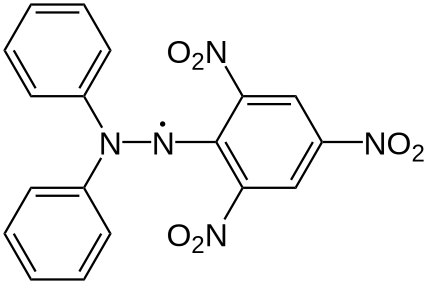
\includegraphics[width=\linewidth]{external/DPPH.pdf}
\end{image}%
Son facteur de Landé est très proche de celui de l’électron libre, avec une valeur typique \(g \approx 2.0036\). C'est une référence particulièrement utile pour l’étalonnage du champ magnétique et la calibration d’un spectromètre RPE. Le spectre se caractérise par une raie unique étroite, dont la largeur est peu dépendante des conditions expérimentales.%
\end{remark}
\end{subsectionptx}
%
%
\typeout{************************************************}
\typeout{Sous-section 3.3 Estimation de \(g\)}
\typeout{************************************************}
%
\begin{subsectionptx}{Sous-section}{Estimation de \(g\)}{}{Estimation de \(g\)}{}{}{subsec-mesure-g}
%
\begin{itemize}[label=\textbullet]
\item{}Proposez une première méthode pour estimer le facteur \(g\) du DPPH. Quelle est la principale source d'erreur ?%
\item{}Pour obtenir d'autres points de mesure, trouvez des modes du KTO à plus haute fréquence et observez à nouveau la résonance.%
\item{}Pour obtenir un point à plus basse fréquence, vous pouvez utiliser le deuxième résonateur en KTO.%
\end{itemize}
%
\end{subsectionptx}
\end{sectionptx}
\end{document}
